\documentclass{article}

\usepackage{url} 

\usepackage{pdfpages}
\usepackage{lastpage}
\usepackage{fancyhdr}
\usepackage{ngerman}


\usepackage{xcolor}
\usepackage{listings}
\usepackage{courier}


\usepackage{floatrow}
\usepackage[tableposition=top]{caption}
\floatsetup[table]{capposition=top}

\usepackage{amsmath, amssymb}

\usepackage[utf8]{inputenc}


\usepackage[numbib]{tocbibind}


\title{Elastizität}
\author{Johannes Winkler}
\date{}


\newcommand\twodigits[1]{%
   \ifnum#1<10 0#1\else #1\fi
}



\lhead{Elastizität}
\rhead{\today\\Johannes Winkler}
\cfoot{\twodigits{\thepage}~/ \pageref{LastPage}}

\begin{document}


\includepdf[page=-]{deckblatt.pdf} 
 
 
\pagestyle{fancy}


\tableofcontents

\newpage


\setcounter{section}{-1}

\section{Experimentiervorschlag}


Ich möchte die Elastizität eines Holzstabes und einer Holzplatte testen. Der Versuchsaufbau wäre folgender:
\begin{figure}[H]
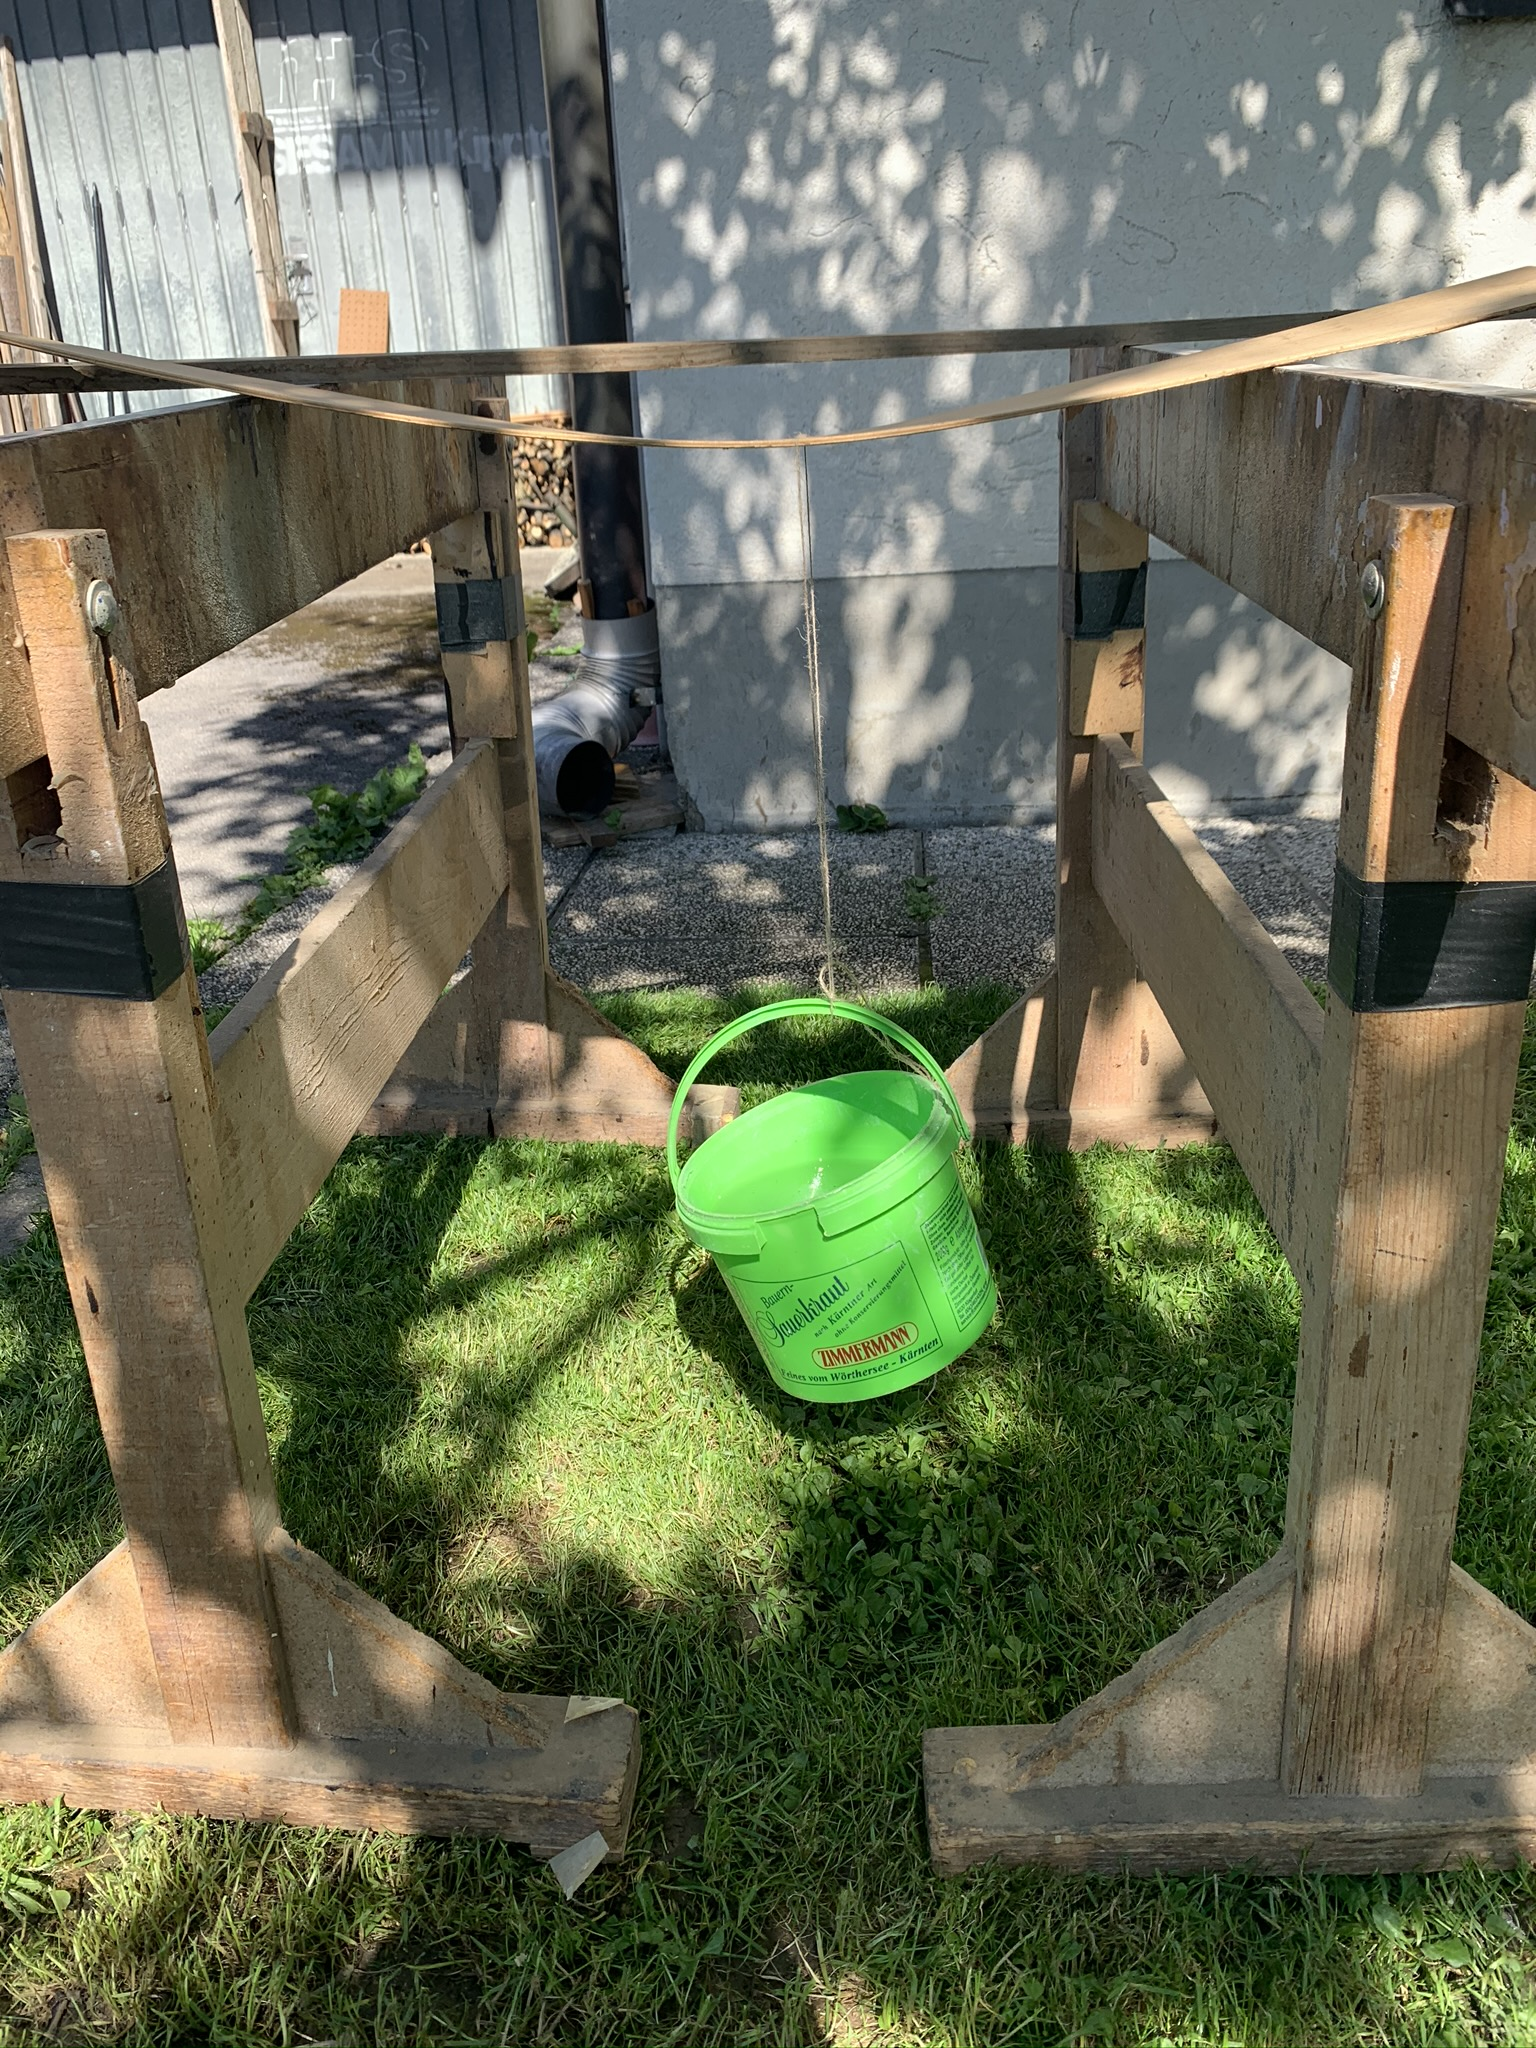
\includegraphics[height=10cm]{aufbau.jpg}
\caption{Versuchsaufbau}
\end{figure}

In den Eimer werden mit Hilfe eines Messbechers Wasser gefüllt. Durch das Gewicht des vollen Eimers biegt sich das Holzbrett immer stärker nach unten. Dadurch kann der E-Modul bestimmt werden.

Um die exakte Menge Wasser zu bestimmen, werde ich sowohl Waage, als auch einen Messbecher verwenden. Die zu verwendende Menge an Wasser wird während des Experiments bestimmt.

Die zu messende Größe ist in der nachfolgenden Skizze eingezeichnet


\newpage

\subsection*{Messvorgang der Durchbiegung:}

Zuerst werde ich schrittweise die Wassermenge im Eimer erhöhen (um eine vorher definierte Menge). Dann werde ich $\Delta h$ messen, indem ich zB. eine Wasserwaage (als Referenz für einen \textit{geraden} Stab) auf die Holzstützen lege und dann mit einem Maßband den senkrechten Abstand zur tiefsten Stelle des gebogenen Stabes messe (aus Symmetriegründen in der Mitte des gebogenen Brettes). Alternativ kann ich auch den Abstand zum Boden messen und durch Subtraktion $\Delta h$ indirekt bestimmen. Welche der beiden Methoden besser ist, möchte ich dann im Experiment prüfen (hängt natürlich vom Untergrund ab und davon ob die Höhe der Stützen exakt ist). Ich werde das genau prüfen und meine Entscheidung numerisch begründen.

Aus dem Experiment erhalte ich dann Zahlentupel $(w_\text{max}, F)$. Diese kann ich nach den gängigen Methoden der Statistik analysieren. Laut Gleichung \eqref{eq:emodul} besteht ein linearer Zusammenhang, hier würde sich zusätzlich eine Regression anbieten. Schließlich lässt sich aus dem linearen Zusammenhang dann der Proportionalitätsfaktor und daraus auch $E$ berechnen.


\begin{figure}[H]
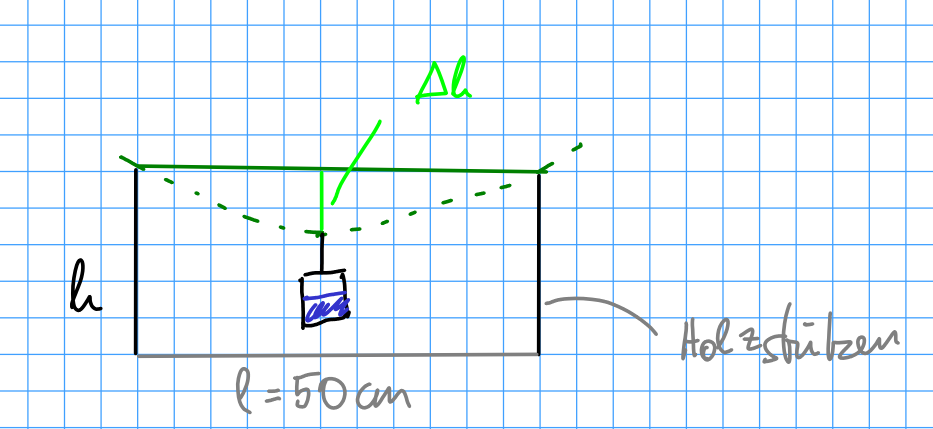
\includegraphics[height=5cm]{skizze.png}
\caption{Gesucht ist $\Delta h$ für ein definertes Gewicht im Eimer.}
\end{figure}


\begin{figure}[H]
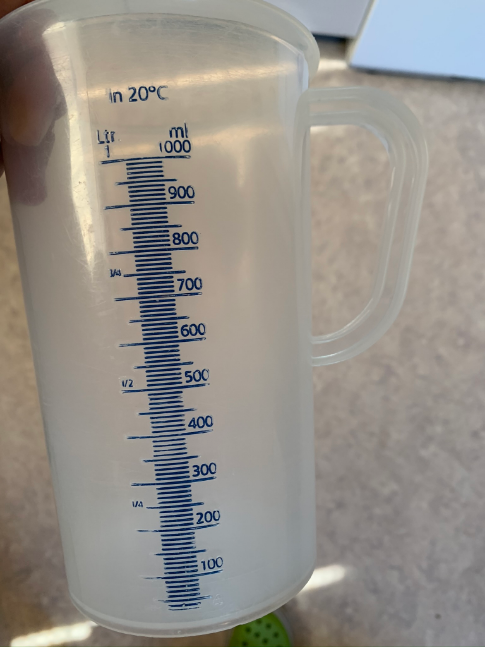
\includegraphics[height=5cm]{messbecher.png}
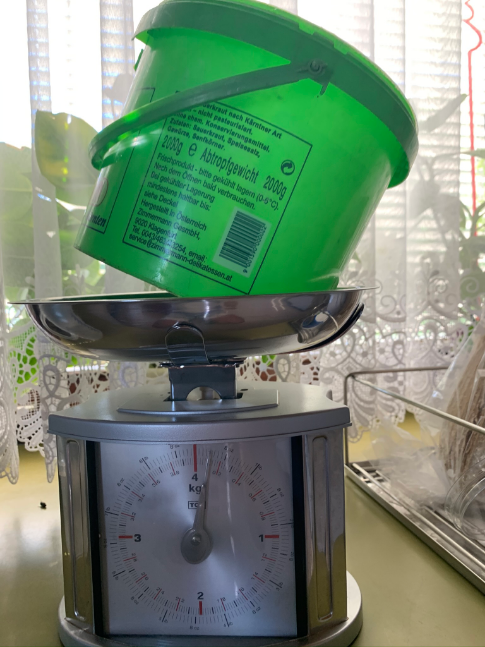
\includegraphics[height=5cm]{eimer_waage.png}
\caption{Waage, Messbecher, Eimer.}
\end{figure}




Als Hilfsmittel verwende ich einige Dinge (siehe Geräteliste), unter anderem meine üblichen Werkzeuge
\begin{figure}[H]
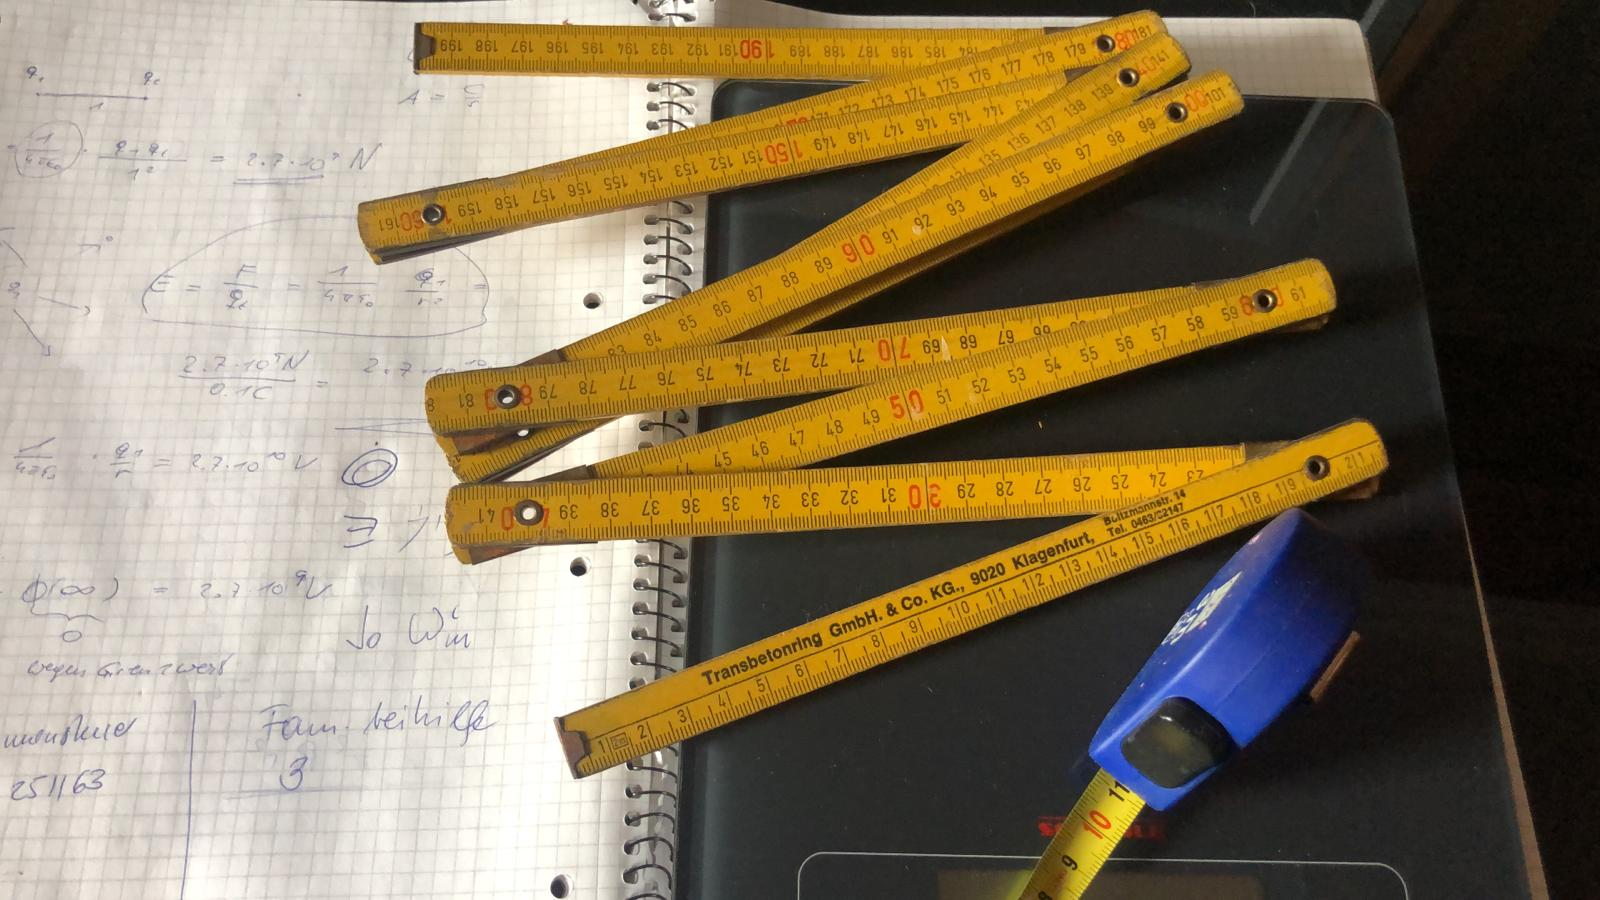
\includegraphics[height=5cm]{zeux.jpg}
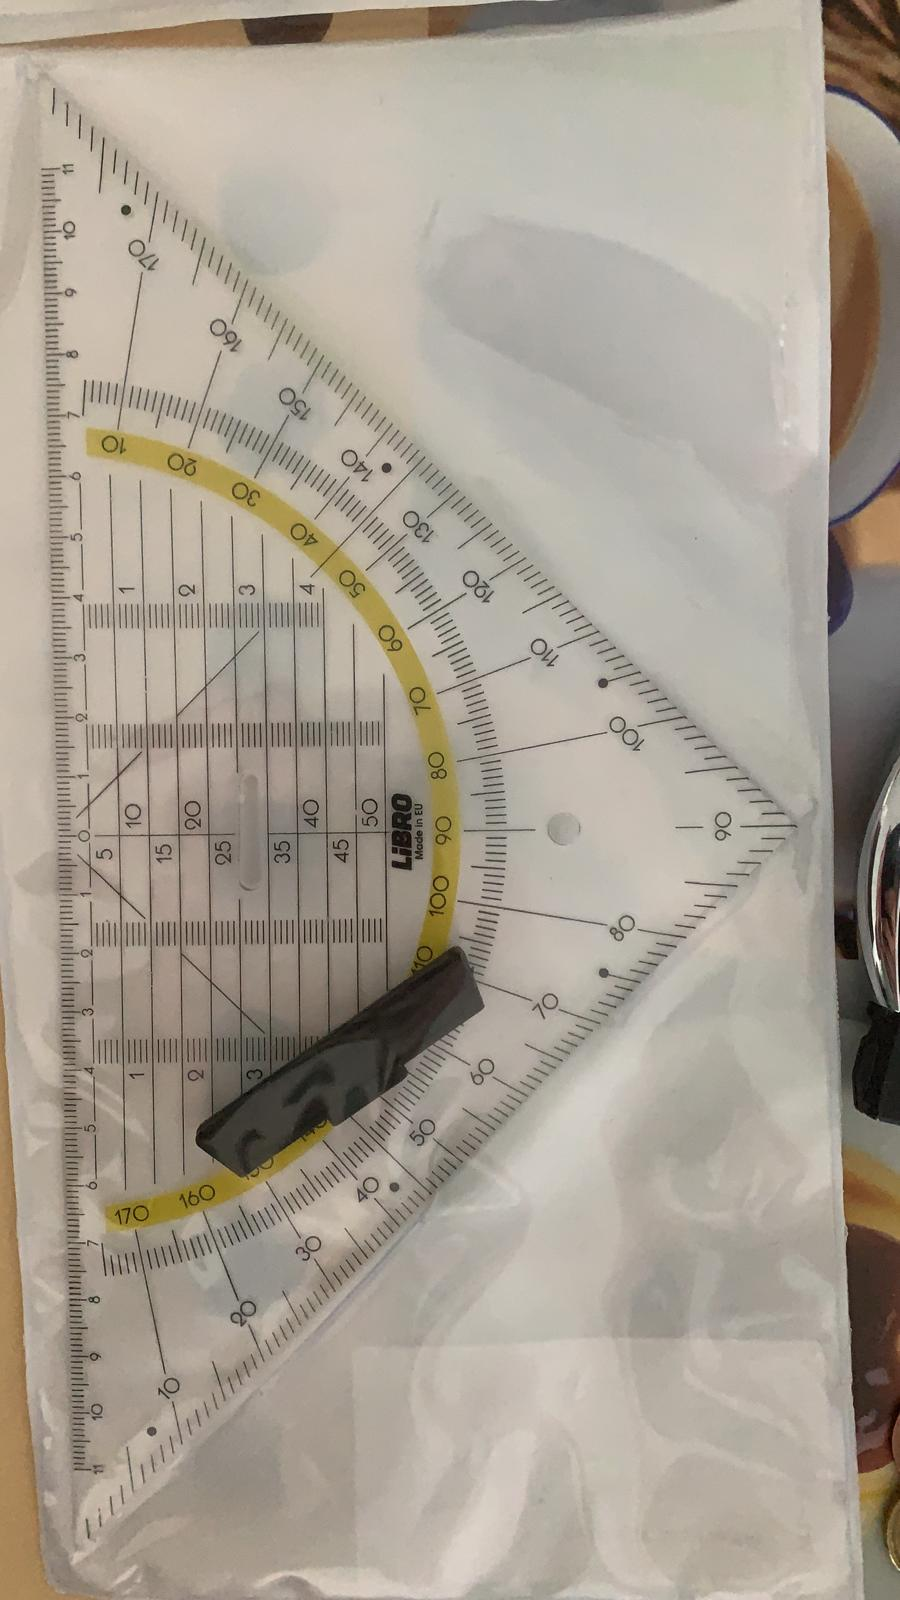
\includegraphics[height=5cm]{lineal.jpg}
\caption{Übliche Messinstrumente, die ich immer verwende.}
\end{figure}

Die Holzplatte und der Holzstab sehen folgend aus
\begin{figure}[H]
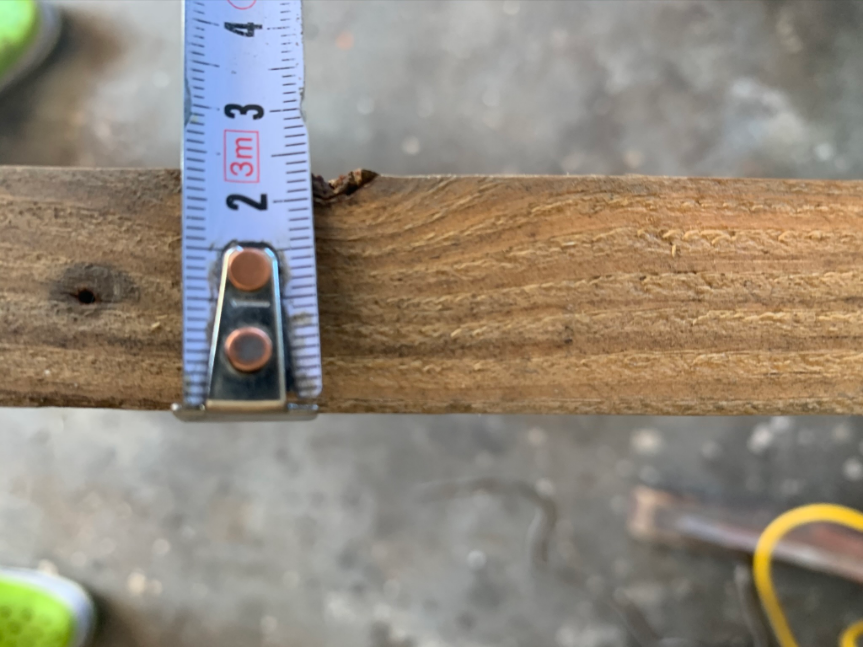
\includegraphics[height=5cm]{stab.png}
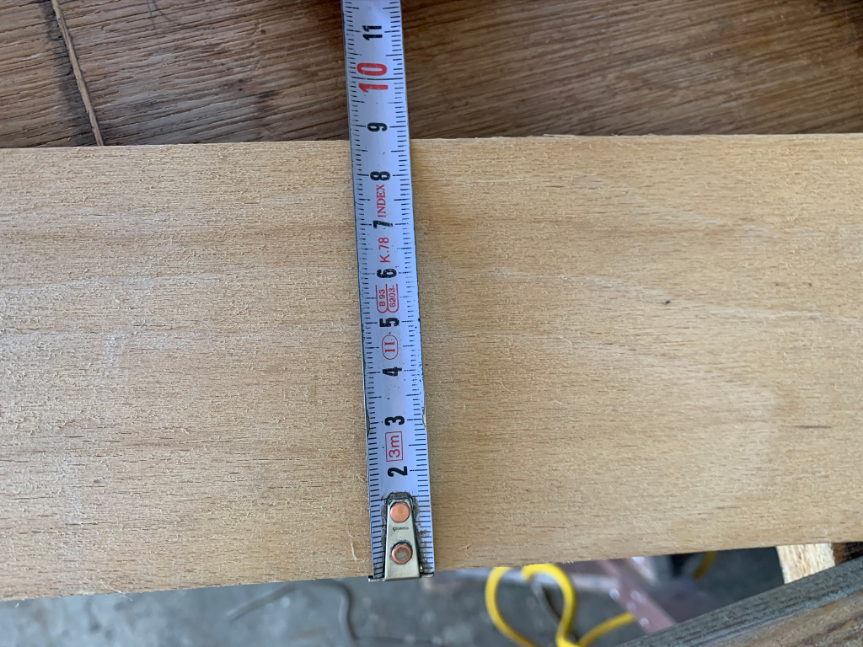
\includegraphics[height=5cm]{platte.png}
\caption{Holzstab und Holzplatte.}
\end{figure}


\begin{figure}[H]
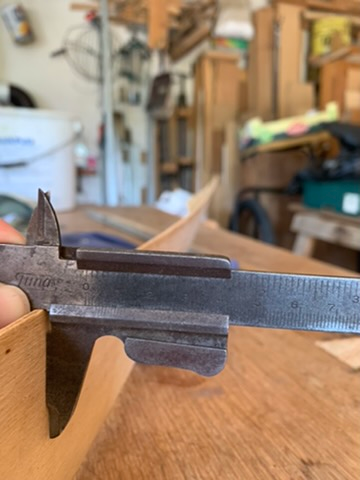
\includegraphics[height=5cm]{schiebelehre.png}
\caption{Schiebelehre.}
\end{figure}



\newpage

\section{Aufgabenstellung}

Es ist der Elastizitätsmodul eines Stabes zu bestimmen. Ich verwende einen Holzstab und eine Holzplatte. Ziel dieses Versuch ist es, herauszufinden, wie sehr die Form eines Stabes Abweichung bei der Bestimmung des Elastizitätsmoduls hervorruft.


\section{Grundlagen}

Wirken auf einen Körper äußere Kräfte, die im Gleichgewicht sind, so tritt eine Änderung der
Form und des Volumens des Körpers ein, die bei Beenden der Kraftwirkung wieder vollständig
zurückgeht, solange die Deformation die Grenze des elastischen Bereiches nicht überschreitet.
Die Dehnung $\epsilon$ (positiv oder negativ) ist dann proportional der wirkenden Spannung $\sigma$. Die Proportionalitätskonstante $E$ (in N/m${}^2$) wird Elasitizitätsmodul genannt.
\begin{align}
\sigma = \epsilon\cdot E
\end{align}
Betrachtet man einen auf zwei Schneiden im Abstand $L$ gelagerten Stab mit einer in der Mitte angreifenden Kraft $F$ bei kleiner Durchbiegung, so ergibt sich die größte Durchbiegung $w_\text{max}$ in der Mitte zu
\begin{align}
\label{eq:emodul}
w_\text{max} = \frac{F\cdot L^3}{48\cdot E \cdot I_y}
\end{align}
$I_y$ ist dabei das Flächenträgheitsmoment des Stabes
\begin{align}
I_y = \int z^2\cdot dA \\
\text{rechteckiges Stabprofil: } I_y = \frac{b\cdot h^3}{12} \\
\text{kreisförmiges Stabprofil: } I_y = \frac{\pi\cdot d^4}{64} 
\end{align}
Die bei der Biegung im Stab auftretende absolut größte Biegespannung $\sigma_b^{\text{max}}$ lässt sich aus dem infolge der angreifenden Kraft auftretenden Biegemoment $M_b$ der Stabhöhe $h$ und dem Biegemoment $M_b$ berechnen.
\begin{align}
\sigma_b^{\text{max}} &= \frac{h\cdot M_b^\text{max}}{2\cdot I_y} \\
M_b^\text{max} &= \frac{F\cdot L}{4} = \frac{m\cdot g\cdot L}{4}
\end{align}


\newpage




\definecolor{commentgreen}{RGB}{2,112,10}
\definecolor{eminence}{RGB}{108,48,130}
\definecolor{weborange}{RGB}{255,165,0}
\definecolor{frenchplum}{RGB}{129,20,83}

\lstdefinelanguage{elixir}{
    morekeywords={def, for, range, abs, return},
    otherkeywords={<-,->, |>, \%\{, \}, \{, \, (, )},
    sensitive=true,
    morecomment=[l]{\#},
    morecomment=[n]{/*}{*/},
    morecomment=[s][\color{purple}]{:}{\ },
    morestring=[s][\color{orange}]"",
    commentstyle=\color{commentgreen},
    keywordstyle=\color{eminence},
    stringstyle=\color{red},
	basicstyle=\ttfamily,
	breaklines,
	showstringspaces=false,
	frame=tb
}

\begin{lstlisting}[language=elixir, caption={Formel zur Berechnung der orthogonalen Regression.},captionpos=b, label=lst:test]
def orthogonal_regression(x,y):
	xd = sum(x)/len(x)
	yd = sum(y)/len(y)
	sx = sum([(a-xd)**2 for a in x])/(len(x)-1)
	sy = sum([(b-yd)**2 for b in y])/(len(y)-1)
	sxy = sum( [ (x[i] - xd)*(y[i]-yd) for i in range(len(x))] )/(len(x)-1)
	beta1 = (sy-sx + sqrt( (sy-sx)**2 + 4*sxy**2))/(2*sxy)
	beta0 = yd - beta1 * xd
	return beta0, beta1
\end{lstlisting}


\section{Beschreibung der Versuchsanordnung}

\begin{figure}[H]
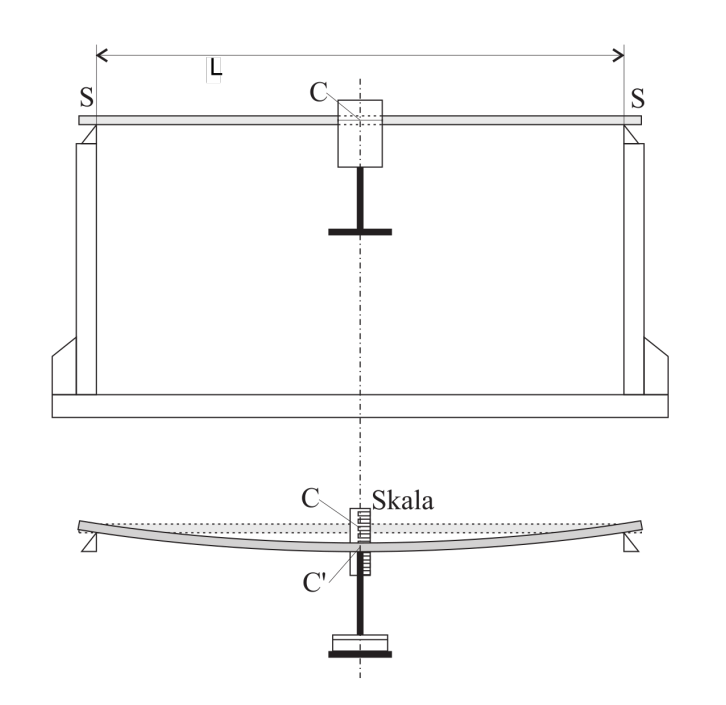
\includegraphics[height=5cm]{versuch.png}
\caption{Versuchsaufbau zur Bestimmung der maximalen Durchbiegung eines Stabes unter
Belastung. $S_1$, $S_2$ Auflagepunkte des Stabes, $L$ Abstand der Auflagepunkte, $C$ Stabmitte im unbelasteten Zustand und Angriffspunkt der Kraft, $C_0$ Stabmitte im belasteten Zustand.}
\end{figure}





\section{Geräteliste}



\begin{table}[H]
\caption{Geräteliste}



\begin{tabular}{lll}
Gerät  & Beschreibung \\
\hline
analoge Küchenwaage & kein Hersteller erkennbar (max. 4 kg) \\
digitale Waage aus Werkstatt & kein Hersteller erkennbar (max. 25 kg) \\
Kamera & iPhone XS Max \\
Maßband &  \\
Holzstab &  $0.8~$cm x $2.4~$cm x $150~$cm \\
Holzbrett & $0.3~$cm x $8.7~$cm x $102~$cm\\
2 Stützen aus Holz & \\
Schiebelehre & \\ 
Schnur & \\
Eimer & 3 Liter Fassungsvermögen\\
Eimer & 10 Liter Fassungsvermögen\\
\end{tabular}
\end{table}

\newpage
\section{Versuchsdurchführung und Messergebnisse}

Ein Holzstab und ein Holzbrett sind auf 2 Stützen im Abstand von $L=0.5~$m aufgelegt. In der Mitte des Stabes bzw. Brettes ist ein Eimer mit Wasser angebracht, sodass eine Kraft auf die Holzstücke wirkt. Die Biegung nach unten relativ zur Ausgangshöhe (mit Wasserwaage normiert) wird in cm gemessen. Für den Holzstab wird sie als $h_1$ und für das Holzbrett als $h_2$ bezeichnet.

Die Wassermenge im Eimer wurde so gewählt, dass Gewicht am Brett von 0 auf 5~kg in 500~g Schritten erfolgt. Da keine Federwaage vorhanden ist, wird das gemessene Gesamtgewicht des Eimers mit $g=9.81~$m/s${}^2$ multipliziert, um die angreifende Kraft $F$ zu erhalten. Es werden also 10 Messungen vorgenommen. Diese sind in Tabelle \ref{tab:messungen} dokumentiert.


\begin{table}[H]
\caption{Tabelle mit den Messungen. Die Masse $m$ wurde mit einer Waage bestimmt, die Kraft $F$ wurde indirekt durch Multiplikation mit der Erdbeschleunigung $g$ berechnet.}
\label{tab:messungen}


\begin{tabular}{ll|ll}
$m$ / kg & $F$ / N & $h_1$ / cm & $h_2$ / cm\\
\hline
0.00	&	0.00	&	0.0	&	0.0\\0.50	&	4.91	&	0.2	&	1.1\\1.00	&	9.81	&	0.4	&	1.5\\1.50	&	14.71	&	0.6	&	2.2\\2.00	&	19.62	&	0.8	&	3.3\\2.50	&	24.53	&	1.0	&	3.7\\3.00	&	29.43	&	1.1	&	4.4\\3.50	&	34.34	&	1.4	&	5.0\\4.00	&	39.24	&	1.5	&	6.2\\4.50	&	44.15	&	1.8	&	7.0\\5.00	&	49.05	&	1.9	&	7.3\\
\end{tabular}

\end{table}

\begin{table}[H]
\caption{Abmessungen der zu Gegenstände.}
\begin{tabular}{l|lll}
& h / cm & b / cm & $\ell$ / cm \\
\hline
Holzstab & 0.8 & 2.4  &  150.0 \\
Holzbrett & 0.3 & 8.7 & 102.0
\end{tabular}
\end{table}






\newpage
\section{Auswertung}

Das Flächenträgheitsmoment ist für rechteckige Querschnitte 
\begin{align}
I_y = \frac{b\cdot h^3}{12}
\end{align}
Die Unsicherheit ist
\begin{align}
\Delta I_y &= \left| \frac{\partial I_y}{\partial b}\right| \cdot \Delta b + \left| \frac{ \partial I_y}{\partial h} \right| \cdot \Delta h \\
&= \frac{\Delta b\cdot h^3}{12} + \frac{3\cdot b\cdot h^2 \cdot \Delta h}{12} = \frac{\Delta b \cdot h^3 + 3\cdot b \cdot h^2 \cdot \Delta h}{12}
\end{align}

Eingesetzt ergibt sich daher 
\begin{align*}
I_{y,\text{Holzstab}} &= (1.024\cdot 10^{-9} \pm 4.267\cdot 10^{-10})~\text{m}^4 \\
I_{y,\text{Holzbrett}} &= (1.956\cdot 10^{-10} \pm 1.980\cdot 10^{-10})~\text{m}^4
\end{align*}
Zusätzlich haben wir $\Delta b = \Delta h = 1~$mm festgelegt.


Für die Auswertung verwenden wir die orthogonale Regression (vgl. \cite{regr} und Listing 1). Der Grund hierfür ist, dass sowohl die $x$- als auch $y$-Koordinate gemessen sind und durch die orthogonale Regression ein potenzieller Messfehler in beiden Koordinatenachsen berücksichtigt wird. Der Algorithmus wurde in Python programmiert und ist in \cite{script} abrufbar. Die Ergebnissen sind ebenfalls aus besagtem Skript nachvollziehbar berechnet.


\begin{figure}[H]
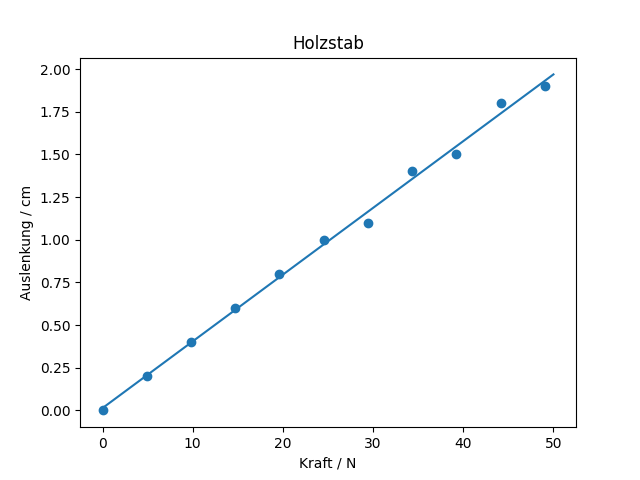
\includegraphics[scale=0.5]{regression1.png}
\caption{Auslenkung des Holzstabes bei einer wirkenden Kraft.}
\end{figure}
\begin{figure}[H]
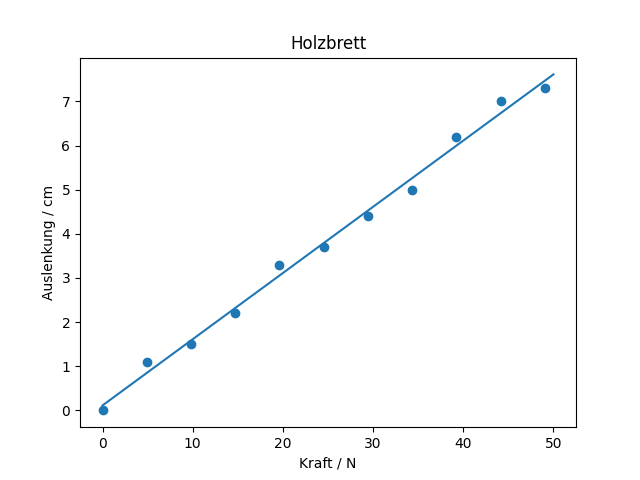
\includegraphics[scale=0.5]{regression2.png}
\caption{Auslenkung des Holzbrettes bei einer wirkenden Kraft.}
\end{figure}

Das Regressionsmodell gibt uns für die Zahlenpaare $(F_i, h_i)$ eine Gerade
\begin{align}
h =  \beta_0 + \beta_1\cdot F
\end{align}
mit minimalen Orthogonalabstand zu den Messpunkten. Im gegebenen Fall sind die Regressionsgeraden
\begin{align*}h_1 &= 0.0136~\text{cm} + 0.0391~\text{cm}/\text{N} \cdot F \\h_2 &= 0.1131~\text{cm} + 0.15~\text{cm}/\text{N} \cdot F \end{align*}

 Sinnvollerweise muss $\beta_1 \approx 0$ ergeben, sonst wäre die direkte Proportionalität verletzt. Aus Formel \eqref{eq:emodul} folgt für $\omega_\text{max} = h$
\begin{align}
h &= F\cdot \underbrace{\frac{ L^3}{48\cdot E \cdot I_y}}_{\beta_1}
\end{align}
Insgesamt gilt dann
\begin{align}
h = \beta_1\cdot F \qquad \text{ mit } \qquad \beta_1 = \frac{L^3}{48\cdot E \cdot I_y}
\end{align}
Für den Elastizitätsmodul folgt daraus
\begin{align}
E &= \frac{L^3}{48\cdot \beta_1 \cdot I_y} \\
\Delta E &= \frac{3\cdot L^2\cdot \Delta L}{48\cdot \beta_1 \cdot I_y} + \frac{L^3\cdot \Delta \beta_1}{48\cdot \beta_1^2 \cdot I_y} + \frac{L^3\cdot \Delta I_y}{48\cdot \beta_1 \cdot I_y^2} \\
&= \frac{L^2}{48\cdot \beta_1\cdot I_y} \cdot \left( 3\cdot \Delta L + L\cdot\frac{\Delta\beta_1}{\beta_1} + L\cdot \frac{\Delta I_y}{I_y}\right)
\end{align}
Durch Einsetzen erhält man die Werte für den Elastizitätsmodul. Wichtig ist hier allerdings, dass man $\beta_1$ vor dem Einsetzen in die Einheit m/N umrechnet. 


Die Bestimmung der Abweichung von $\beta_1$ ist mathematisch nicht trivial. Bei der Bestimmung geht man davon aus, dass die Randpunkte die Regressionsgerade stärker beeinflussen. Verschiebt man bildlich gesprochen den letzten Messpunkt nach \textit{links oben} und den zweiten (weil der erste ist $(0,0)$) nach \textit{rechts unten}, dann rotiert die Regressionsgerade gegen den Uhrzeigersinn und man erhält eine obere Schranke für die Steigung. Rotiert man die Regressionsgerade auf dieselbe Art in die entgegen gesetzte Richtung, so erhält man eine untere Schranke für die Steigung. Die Differenz daraus kann als Fehler $\Delta\beta_1$ verwendet werden.


Es gilt
\begin{align}
\Delta \beta_1 &= \frac{ (h_\text{last} + \Delta h) - (h_2 - \Delta h)}{(F_\text{last} -\Delta F)  - (F_2 + \Delta F)} - \frac{ (h_\text{last} - \Delta h) - (h_2 + \Delta h)}{(F_\text{last} +\Delta F)  - (F_2 - \Delta F)} \\
&= \frac{ h_\text{last} - h_2 + 2\cdot \Delta h}{F_\text{last} - F_2 - 2\cdot \Delta F} - \frac{ h_\text{last} - h_2 - 2\cdot \Delta h}{F_\text{last} - F_2 + 2\cdot \Delta F}
\end{align}

Zusätzlich gilt $\Delta h = 1~$mm und $\Delta F = 0.01~$N.

\newpage
\section{Zusammenfassung und Diskussion}

Es kann durch die grafische Auswertung gezeigt werden, dass bei der Kraftwirkung auf Holzstab und Holzbrett das Hook'sche Gesetz wirkt. 

Der Elastizitätsmodul hat jedoch keinen globalen Referenzwert, da es sehr stark von der Beschaffenheit des Holzes (zB. Fasern, Alter etc) abhängig ist.

Es gilt
\begin{align*}E_\text{Holzstab} &= (6503 \pm 4261)~\text{MPa} \\E_\text{Holzbrett} &= (8871 \pm 9570)~\text{MPa}\end{align*}

Laut Online-Recherche erfährt man, dass der Elastizitätsmodul von Holz im Bereich von ca. 10 bis 15 GPa liegt. Mit der berechneten Unsicherheit liegen die Ergebnisse in der richtigen Größenordnung.

\begin{thebibliography}{9}
\bibitem{demtr1} W. Demtröder, \emph{Experimentalphysik 1: Mechanik und Wärme}, Springer-Spektrum, 8. Auflage, 2018.

\bibitem{giancoli} D. Giancoli, \emph{Physik}, Pearson, 4. Auflage, 2019.

\bibitem{script} \url{https://github.com/jowin202/lab_tugraz/kfu_el.py} (Stand: \today)

\bibitem{regr} \url{https://de.wikipedia.org/wiki/Orthogonale_Regression} (Stand: \today)

\end{thebibliography}

\end{document}
